\documentclass{beamer}
\usepackage{ctex, hyperref}
% \usepackage[T1]{fontenc}
\usepackage{amssymb}
% other packages
\usepackage{latexsym,amsmath,xcolor,multicol,booktabs,calligra, color}
\usepackage{graphicx,pstricks,listings,stackengine}
\usepackage{soul, bookmark}
\usepackage{fontspec}




\author{林嘉恩}
\title{Lowcomote}
\subtitle{RS \& Monitoring for LCDP}
\institute{清华大学}
\date{\today}
\usepackage{Tsinghua}


\sethlcolor{yellow}
% \setmainfont{Times New Roman}
\usepackage{amsmath, fontspec}
\usefonttheme{serif}
% defs
\def\cmd#1{\texttt{\color{red}\footnotesize $\backslash$#1}}
\def\env#1{\texttt{\color{blue}\footnotesize #1}}
\definecolor{deepblue}{rgb}{0,0,0.5}
\definecolor{deepred}{rgb}{0.6,0,0}
\definecolor{deepgreen}{rgb}{0,0.5,0}
\definecolor{halfgray}{gray}{0.55}

\lstset{
    basicstyle=\ttfamily\small,
    keywordstyle=\bfseries\color{deepblue},
    emphstyle=\ttfamily\color{deepred},    % Custom highlighting style
    stringstyle=\color{deepgreen},
    numbers=left,
    numberstyle=\small\color{halfgray},
    rulesepcolor=\color{red!20!green!20!blue!20},
    frame=shadowbox,
}


\begin{document}
% 首页
\kaishu
\begin{frame}
    \titlepage
    \begin{figure}[htpb]
        \begin{center}
            
\includegraphics[width=0.2\linewidth]{pic/Tsinghua_University_Logo.eps}
        \end{center}
    \end{figure}
\end{frame}
%目录
\begin{frame}
    \tableofcontents[sectionstyle=show,subsectionstyle=show/shaded/hide,subsubsectionstyle=show/shaded/hide]
\end{frame}



\section{研究领域概览: RS in MDE},

\subsection{timeline}
\begin{frame}{Lissette Almonte Garcia}
    \begin{itemize}
        \item 2020年发了第一篇关于自动生成推荐系统集成到MDE中的文章,相对来说只是理论为主。
        \begin{itemize}
            \item \textit{Towards automating the construction of recommender systems for low-code development platforms} 
        \end{itemize}
        \item 2021年把之前的工作集成到了eclipse以外的平台进行测试
        \begin{itemize}
            \item \textit{Automating the Synthesis of Recommender Systems for Modelling Languages} 
        \end{itemize}
        \item 2022年在RS配置中加入数据预处理
        \begin{itemize}
            \item \textit{Building recommender systems for modelling languages with DROID} 
        \end{itemize}
        \item 2022年发表了一篇综述,虽然对这项工作没有什么特别的改进,但是可以帮助我们系统地认知这个领域
        \begin{itemize}
            \item \textit{Recommender Systems in Model-Driven Engineering} 
        \end{itemize}
    \end{itemize}
\end{frame}

\subsection{Research Questions}
\begin{frame}{Research Questions}
    \begin{enumerate}
        \item In \textbf{which ways} can recommender systems assist in the different tasks within MDE processes?
        \begin{itemize}
            \item complete and repair artefacts, and work over models
        \end{itemize} 
        \item \textbf{Which recommendation} techniques are most commonly used to support MDE tasks, and \textbf{how} are recommenders for MDE \textbf{evaluated}?
        \begin{itemize}
            \item knowledge-based followed by content-based
            \item offline experiments
        \end{itemize}
        \item What are the \textbf{main opportunities} in recommender systems for MDE solutions?
        \begin{itemize}
            \item model transformations or code generators
            \item creating, reusing or finding artefacts
            \item effective repositories of MDE artefacts that mitigate the current lack of data
            \item adapting RSs to the user's needs
            \item mechanisms to exploit the crowd knowledge via collaborative filtering
            \item the userbased evaluation of RSs within MDE
            \item effective integration of RSs with MDE tools and low-code platforms
        \end{itemize}
    \end{enumerate}
\end{frame}

\subsection{dimensions}
\begin{frame}{Dimensions}
    \begin{figure}
        \centering
        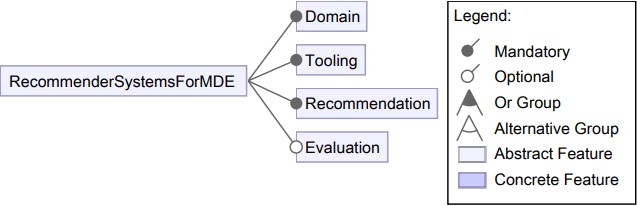
\includegraphics[width = \linewidth]{RS4MDE-pic/4dimensions.jpg}
        \caption{Dimensions for analysing the use of RSs in MDE.}
    \end{figure}
    文章分了四个维度来叙述模型驱动工程中的推荐系统,分别是推荐系统在什么领域解决什么问题、提出的工具有什么特点、使用到了什么样的推荐系统以及怎么评价这个推荐系统。
\end{frame}

\subsection{domain}
\begin{frame}{RS in MDE: domain}
    \begin{figure}
        \centering
        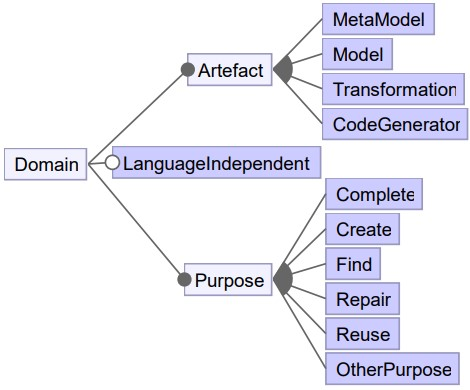
\includegraphics[width = 0.6\linewidth]{RS4MDE-pic/domain.jpg}
        \caption{Domain dimensions for RSs in MDE.}
    \end{figure}
    重点关注:Complete
\end{frame}
% \begin{frame}{RS in MDE: domain}
%     \begin{itemize}
%         \item Complete 完成模型
%         \begin{itemize}
%             \item 使用搜索技术扩展部分模型形成完整模型
%             \item 给出一个模型逐步完成的建议
%         \end{itemize}
%         \item Create 创建模型
%         \begin{itemize}
%             \item 相对较少,只有两个,分别针对模型和元模型
%         \end{itemize}
%         \item Find 查找工件
%         \begin{itemize}
%             \item 查找模型工件。从(异构)库中查找并根据用户适用性排序
%         \end{itemize}
%         \item Repair 修复工件
%         \begin{itemize}
%             \item 修复工件,检查错误
%         \end{itemize}
%         \item Reuse 复用
%         \begin{itemize}
%             \item 不只是查找,在新的上下文中提供复用工件的帮助。
%         \end{itemize}
%     \end{itemize}
% \end{frame}


\subsection{tooling}
\begin{frame}{RS in MDE: tooling}
    \begin{figure}
        \centering
        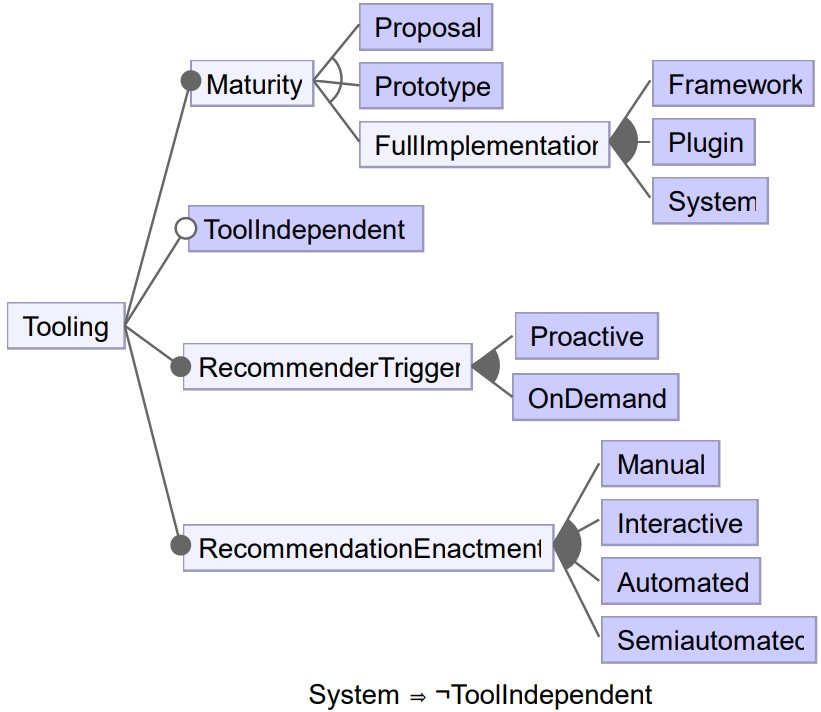
\includegraphics[width = 0.7\linewidth]{RS4MDE-pic/tooling.jpg}
        \caption{Tooling dimensions for RSs in MDE.}
    \end{figure}
    % 目标:Full implement、user demand、interactively
\end{frame}


\subsection{recommendation}
\begin{frame}{RS in MDE: recommendation}
    \begin{figure}
        \centering
        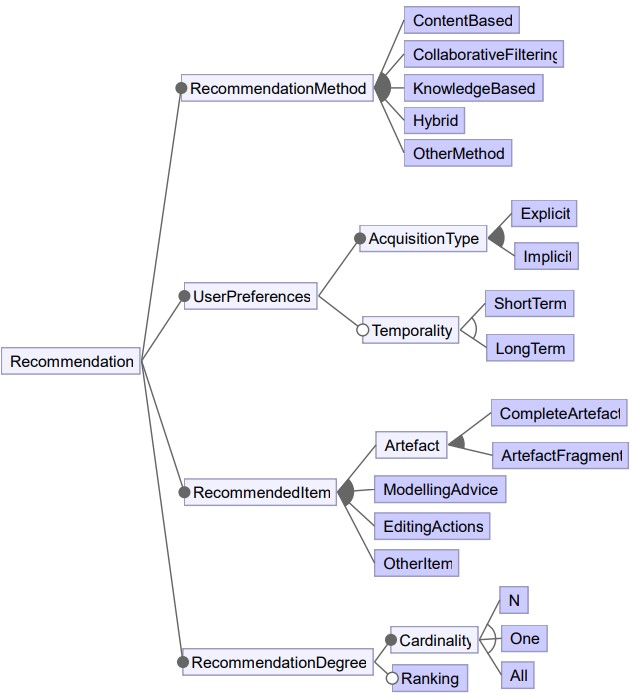
\includegraphics[width = 0.55\linewidth]{RS4MDE-pic/recommendation.jpg}
        \caption{Recommendation dimensions for RSs in MDE.}
    \end{figure}
\end{frame}

\subsection{Evalution}
\begin{frame}{RS in MDE: Evalution}
    \begin{figure}
        \centering
        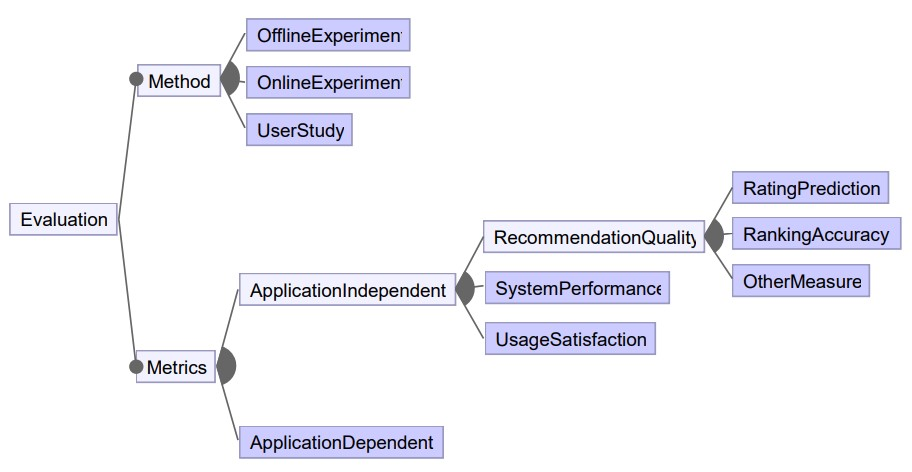
\includegraphics[width = 0.9\linewidth]{RS4MDE-pic/evaluation.jpg}
        \caption{Evaluation dimensions for RSs in MDE.}
    \end{figure}
\end{frame}

\begin{frame}{RS in MDE: Evalution}
    \begin{itemize}
        \item Offline Experiment (4种数据来源)
        \begin{itemize}
            \item 生成数据
            \item 从现成的库中获取数据($\checkmark$)
            \item 从现有文章中获取实例
            \item 从公司获取现实世界的数据
        \end{itemize}
        \item Online Experiment 在线实验 (和A/B测试的差异?)
        \item User Study 用户研究 (三种类型)
        \begin{itemize}
            \item 使用RS来完成任务
            \item 用户在A/B测试中使用RS
            \item 将推荐的项目和专家推荐的对比
        \end{itemize}
    \end{itemize}
\end{frame}
\begin{frame}{RS in MDE: Evalution}
    \begin{itemize}
        \item precision: percentage of the recommended items relevant
        \item recall: percentage of relevant items included in the recommendation list
        \item F1: a harmonic mean of previous two
        \item USC: percentage of users that the RS can recommend
        \item ISC: popularity of what is recommended
        \item nDCG: whether the most relevant items are top
    \end{itemize}
\end{frame}


\section{建模: Auto Generating RS for LCDP}
\subsection{2020: Towards automating the construction of recommender systems for low-code development platforms}


\begin{frame}{Motivating example}
    \begin{itemize}
        \item class modeling
        \begin{figure}[htpb]
            \centering
            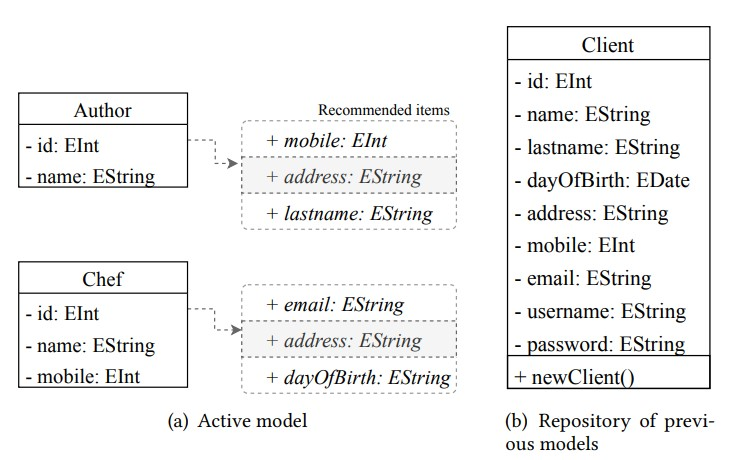
\includegraphics[width=0.7\linewidth]{pic/目标例子.jpg}
            \caption{ Motivating example.}
        \end{figure}
        \item other LCDPs may use alternative modelling notations, and the recommendation task may be different as well
    \end{itemize}
\end{frame}


\begin{frame}{Background: Recommender System}
    \begin{itemize}
        
        
        \item Matrices
        \begin{columns}
            \column{0.5\textwidth}
            \begin{itemize}
            \item \textbf{user-item matrix}:rating given by the user u to the item i
            \item \textbf{item-feature matrix}: each cell is set to 1 if the item has the feature, and to 0 otherwise
            \end{itemize}
            \column{0.5\textwidth}
            \begin{figure}[p]
                \centering
                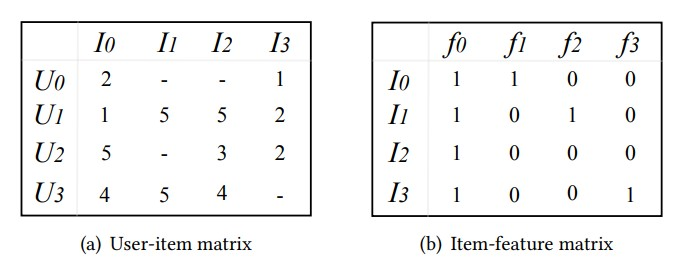
\includegraphics[width=\linewidth]{pic/推荐系统两个矩阵.jpg}
                \caption{Examples of matrices used in RSs.}
            \end{figure}
        \end{columns}
        
    \end{itemize}
    
    
\end{frame}



\begin{frame}{Proposed Approach: Overview of Architecture}
    \begin{columns}
        \column{0.6\textwidth}
        \begin{enumerate}[1]
            \item designer provides the meta-model(class diagram)
            \item repository of models(data)
            \item designer uses a textual DSL to define the meta-model elements
            \item framework will generate a tailored RS for the LCDP
            \item developers will be offered the recommendations within the LCDP environment
            \begin{itemize}
                \item tips over the diagram elements
                \item example fragments
                \item query-answer chatbots addressed in natural language
            \end{itemize}
        \end{enumerate}
        \column{0.4\textwidth}
        \begin{figure}[p]
            \centering
            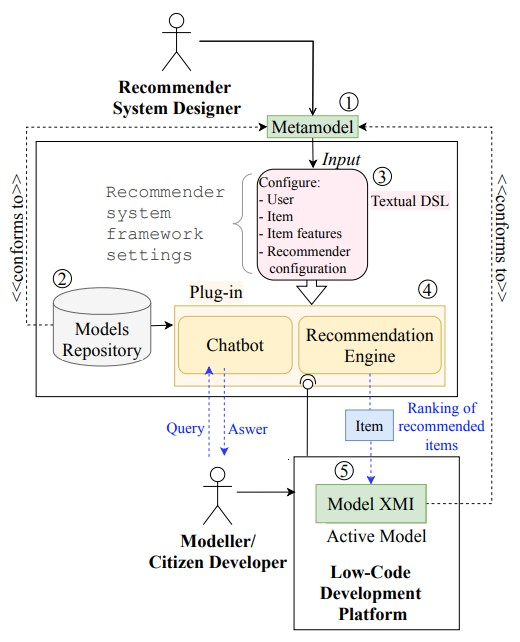
\includegraphics[width=\linewidth]{pic/overview.jpg}
            \caption{ Overview of the proposed approach.}
        \end{figure}
    \end{columns}
\end{frame}

\begin{frame}{Proposed Approach: DSL(step 1-2)}
    \begin{columns}
        \column{0.5\textwidth}
        \begin{figure}[tpb]
            \centering
            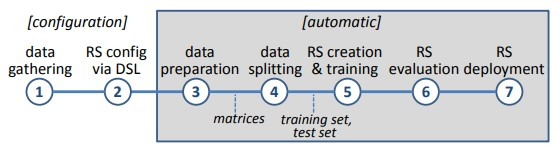
\includegraphics[width=0.8\linewidth]{pic/overview of process.jpg}
            \caption{ Overview of process.}
        \end{figure}
        \begin{figure}[tpb]
            \centering
            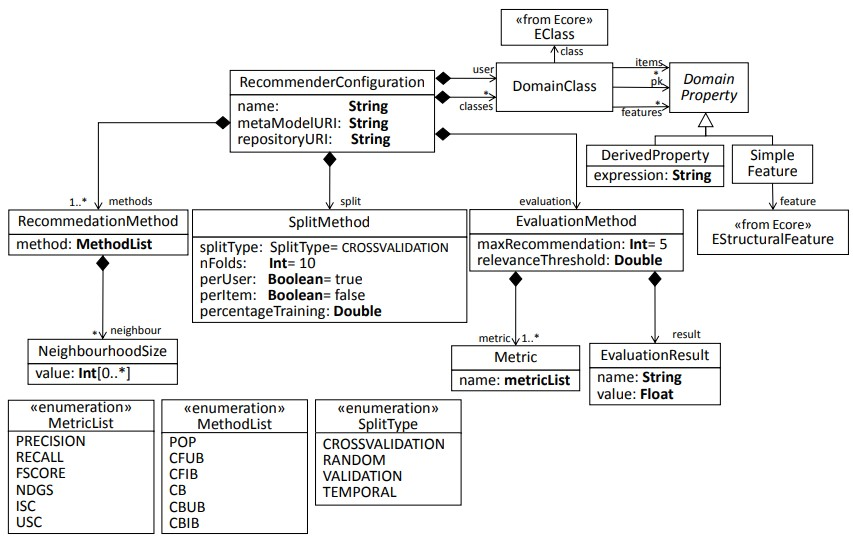
\includegraphics[width=\linewidth]{pic/DSL meta-model.jpg}
            \caption{ Meta-model of the DSL.}
        \end{figure}
        \column{0.5\textwidth}
        \begin{figure}[tpb]
            \centering
            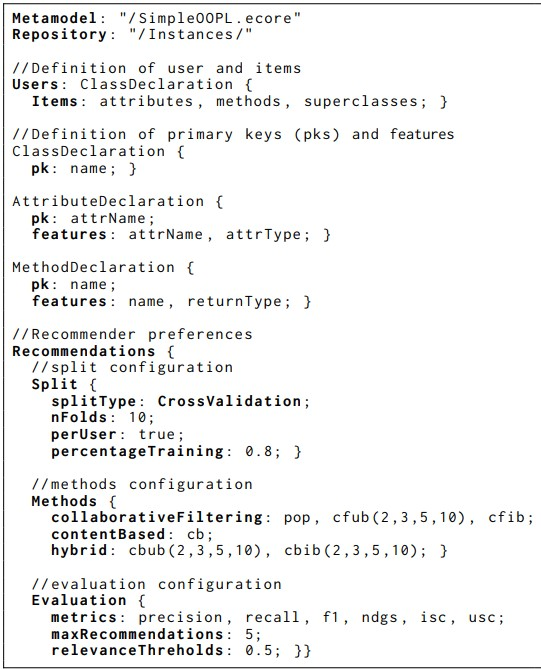
\includegraphics[width=0.9\linewidth]{pic/DSL.jpg}
            \caption{ Example of recommender system configuration.}
            \label{DSL}
        \end{figure}
    \end{columns}
\end{frame}

\begin{frame}{Proposed Approach: Data preparation(step 3)}
    \begin{columns}
        \column{0.5\textwidth}
        \begin{figure}[htbp]
            \centering
            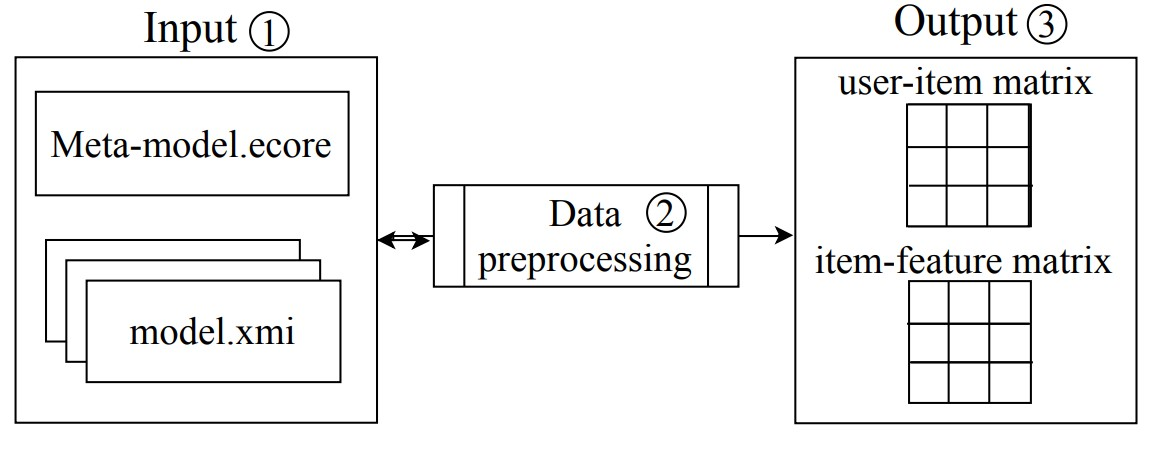
\includegraphics[width = 0.8\linewidth]{pic/数据预处理.jpg}
            \caption{Data preparation steps.}
        \end{figure}
        \begin{enumerate}
            \item retrieves the collection of models
            \item extracts the model objects
            \item generates a user-item matrix and an item-feature matrix
        \end{enumerate}
        \column{0.5\textwidth}
        
        \begin{figure}[htbp]
            \centering
            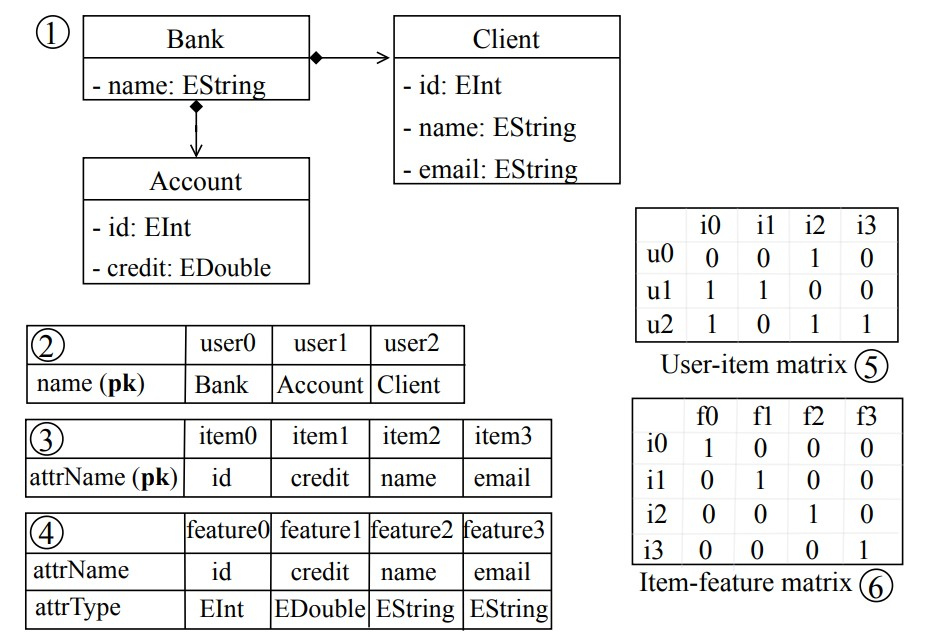
\includegraphics[width = 1.1\linewidth]{pic/数据预处理例子.jpg}
            \caption{Example of data preparation.}
        \end{figure}
    \end{columns}
\end{frame}
    
\begin{frame}{Proposed Approach: Recommendation engine(step4 -7)}
    \begin{figure}[htbp]
        \centering
        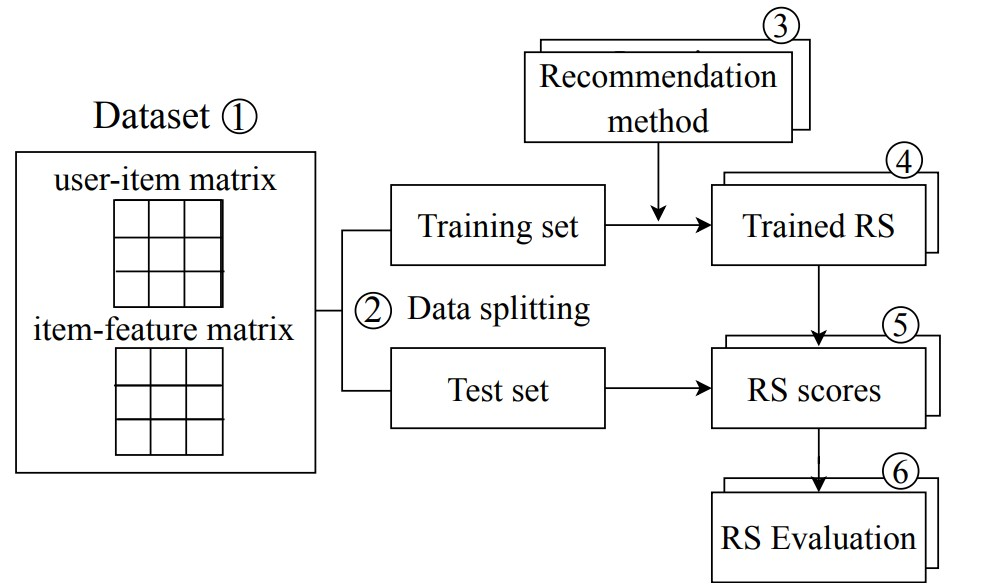
\includegraphics[width = 0.7\linewidth]{pic/RS引擎.jpg}
        \caption{ Steps to build the recommendation engine.}
    \end{figure}
    each candidate RS is evaluated according to the specified metrics, and the results are made available for the designer inspection
\end{frame}

\begin{frame}{Experiment: Setup}
    \begin{itemize}
        \item Dataset
        \begin{itemize}
            \item Synthetic: classes from the Internet
            \item SyntheticExtended: extend first one by synonyms
            \item AtlanEcore: 300 Ecore meta-models
        \end{itemize}
        \item configuration: first two are \ref{DSL}, last one is similar to it
        \item data splitting: 10-fold cross-validation, 8:2 
        \item recommendation methods: top 5
        \begin{itemize}
            \item \textbf{collaborative filtering}: cfubk, cfibk, pop(baseline)
            \item \textbf{content-based}: cb
             \textbf{hybrid}: cbubk
        \end{itemize}
        \item evalution metrics(ranking-based)
        \begin{itemize}
            \item precision、recall、F1、 USC、ISC、 nDCG
        \end{itemize}
    \end{itemize}
\end{frame}

\begin{frame}{Experiment: Result}
    \begin{figure}
        \centering
        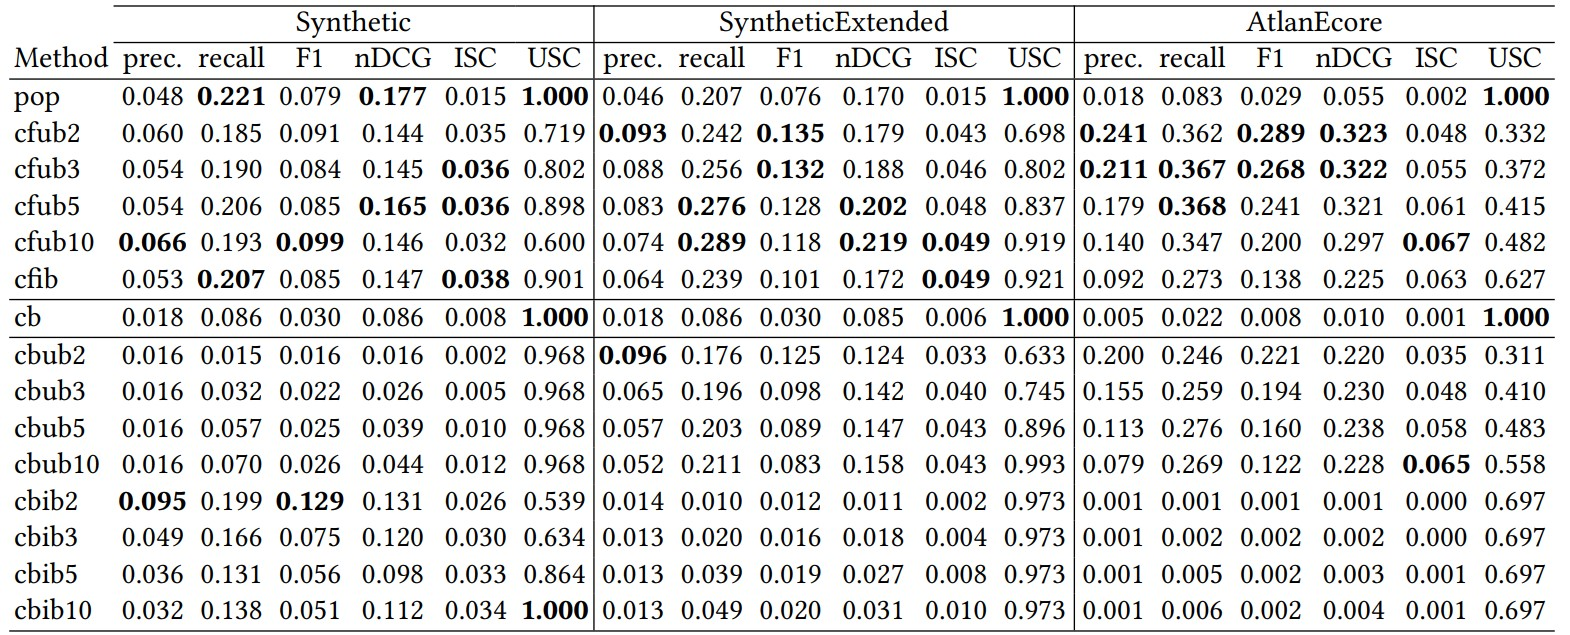
\includegraphics[width = \linewidth]{pic/实验结果.jpg}
        \caption{Results of the experiment. }
    \end{figure}
    \begin{itemize}
        \item The AtlanEcore dataset has the best overall performance.
    \end{itemize}
\end{frame}

\begin{frame}{Experiment: Research Object}
    \begin{enumerate}
        \item Can a recommender system help in class modelling tasks?
        \begin{itemize}
            \item the highest F1 value was 0.289
            \item paper told us it can build an RS that helps in class modelling
        \end{itemize}
        \item Which recommendation method of relevant attributes, methods and superclasses has the best performance?
        \begin{itemize}
            \item SyntheticExtended and AtlanEcore: cfub2, pop has high USC but low ISC
            \item Synthetic: cbib2
        \end{itemize} 
        \item Can hybrid approaches be beneficial for the recommendation of attributes, methods and superclasses?
        \begin{itemize}
            \item in Synthetic, hybrid method has the better result
        \end{itemize}
        \item Which method performs better when considering user and item coverage in the recommendation of relevant attributes, methods and superclasses?
        \begin{itemize}
            \item the methods having low precision and recall report high USC and low ISC
        \end{itemize}
    \end{enumerate}
\end{frame}

\begin{frame}{Personal Thinking}
    \begin{itemize}
        \item how to build
        \begin{itemize}
            \item experiment shows that RS perform well in modeling work, but it's just a framework
            \item writting this driver software is a easy job using RankSys
        \end{itemize}
        \item how to use in DWF
        \begin{itemize}
            \item while customizing form or application, 
            we hope DWF can offer us some advise
        \end{itemize}
        \item the diffculty in building RS for DWF
        \begin{itemize}
            \item \textbf{Data}: each user may have a little model
            \item \textbf{User Similarity}: difference between users is large
            \item \textbf{Result}: we don't know how it perform in DWF area
        \end{itemize}
    \end{itemize}
\end{frame}
% % \section{Auto Generating RS for LCDP 2021}
% % \subsection{2021: Automating the Synthesis of Recommender Systems for Modelling Languages}

% % \begin{frame}{difference in Proposed Approach}
% %     \begin{figure}[htbp]
% %         \centering
% %         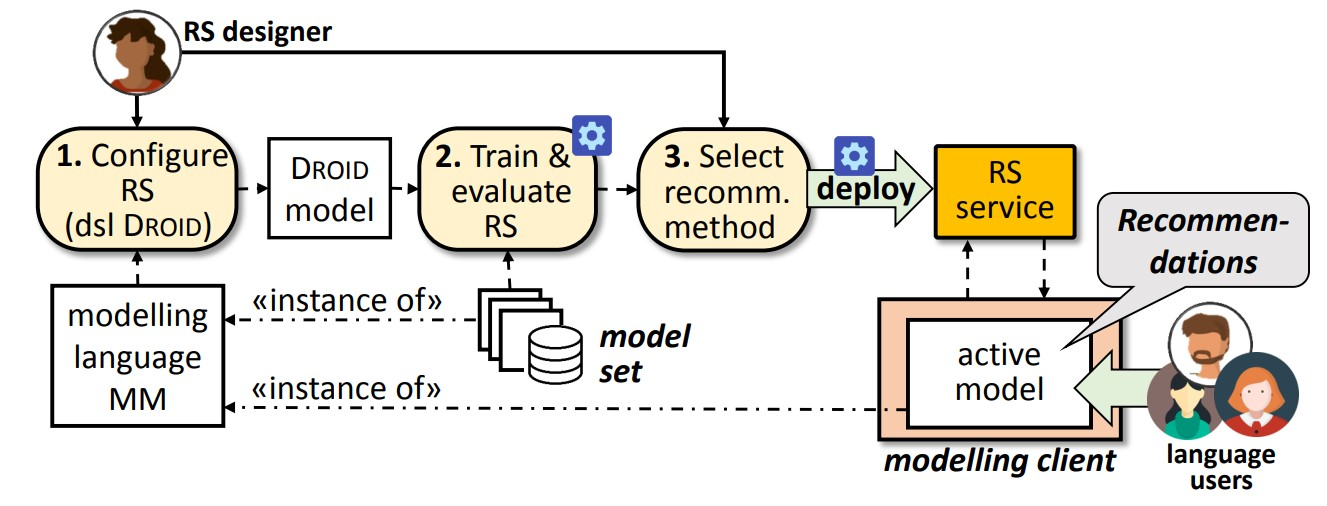
\includegraphics[width=0.7\linewidth]{pic/overview of approach2.jpg}
% %         \caption{Overview of approach.}
% %     \end{figure}
% %     \begin{itemize}
% %         % \item the picture maybe better?
% %         \item it states that designer should choose the method deployed \textbf{in picture}
% %         \begin{itemize}
% %             \item Actually, it has been proposed in text in the previous one.
% %         \end{itemize} 
% %         \item DSL has its own name——DROID and it become more normative.
% %     \end{itemize}
% % \end{frame}

% % \begin{frame}{Tool Support}
% %     \begin{itemize}
% %         \item Configurator: \href{https://droid-dsl.github.io/\#demo}{demo} 
% %         \item The Droid service
% %         \begin{itemize}
% %             \item Recommender: handles the requests from clients
% %             \item ContextItem: parses the received JSON files to extract the recommendation target and its items from the modelling context
% %             \item RecommenderGenerator: generates the recommendations
% %         \end{itemize}
% %         \item Integration with EMF tree editor: client using EMF
% %         \begin{itemize}
% %             \item right click item->choose type->send item and its context->get recommending list
% %         \end{itemize}
% %     \end{itemize}
% %     There is a problem that I can't find any runable example about it. 
% %     The official page just provides some picture. The github repository just provides dataset and result.
% % \end{frame}
% % \begin{frame}{Chatbot}
% %     \begin{columns}
% %         \column{0.5\textwidth}
% %         \begin{figure}
% %             \centering
% %             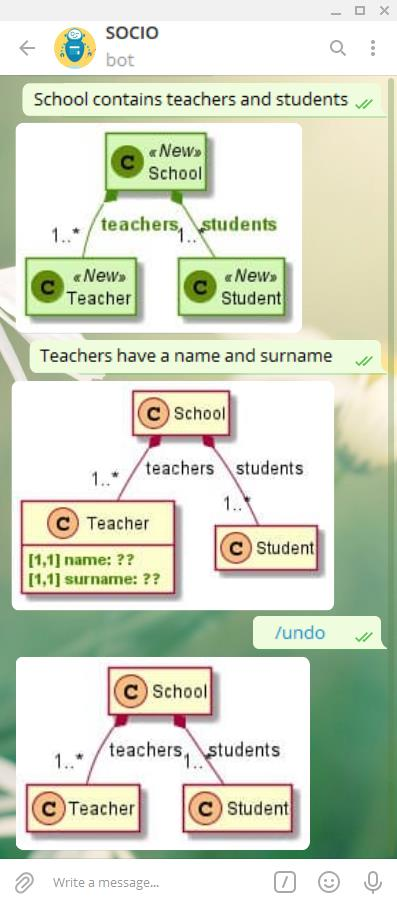
\includegraphics[width = 0.5\linewidth]{pic/效果图.jpg}
% %         \end{figure}
% %         \column{0.5\textwidth}
% %         \begin{figure}
% %             \centering
% %             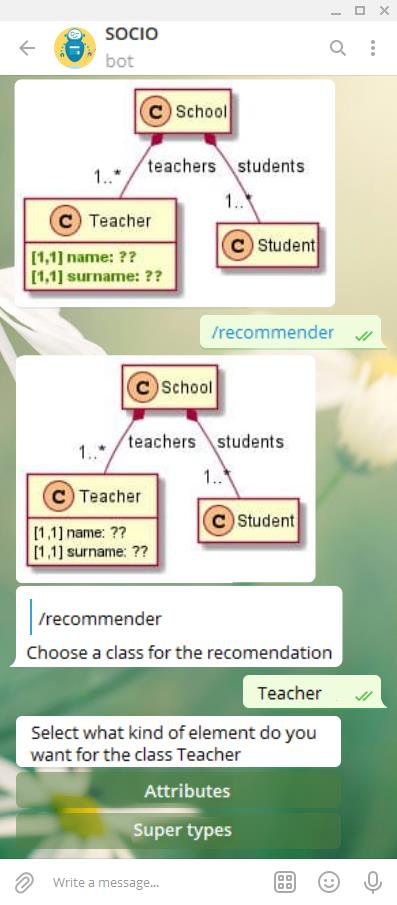
\includegraphics[width = 0.5\linewidth]{pic/效果图2.jpg}
% %         \end{figure}
% %     \end{columns}
    
% % \end{frame}
% % \begin{frame}{Experiment}
% %     \begin{itemize}
% %         \item usefulness experiment
% %         \item integrate RS with a chatbot(how difficult is it to integrate with tools outside Eclipse)
% %         \begin{itemize}
% %             \item Architecture
% %             \begin{figure}
% %                 \centering
% %                 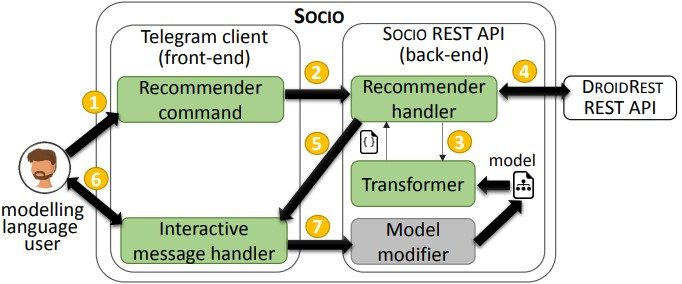
\includegraphics[width = 0.7\linewidth]{pic/architecture of integration.jpg}
% %                 \caption{Architecture of Droid integration with Socio.}
% %             \end{figure}
% %             \item Metrics
% %             \begin{figure}
% %                 \centering
% %                 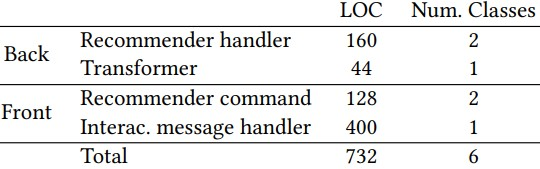
\includegraphics[width = 0.5\linewidth]{pic/LOC.jpg}
% %                 \caption{Metrics for integrating Droid with Socio.}
% %             \end{figure}
% %         \end{itemize}
% %     \end{itemize}
% % \end{frame}
\section{运维:Monitoring ML Model Performance}
\begin{frame}{Panagiotis Kourouklidis}
    \begin{itemize}
        \item 2019年微软发的一篇关于ML中的软工的文章中提到了机器学习工作流的九个阶段,其中包括了Model Monitoring
        \begin{itemize}
            \item \textit{Software Engineering for Machine Learning: A Case Study}
        \end{itemize}
        \item 2020年Panagiotis Kourouklidis发表了第一篇关于自动生成监控系统的文章,主要是说了一下目前ML模型部署后面临的问题以及他的研究计划
        \begin{itemize}
            \item \textit{Towards a low-code solution for monitoring machine learning model performance}
        \end{itemize}
        \item 2021年Panagiotis Kourouklidis发表了第二篇相关文章,提出了一个原始的元模型,并基于Kubernete给出了实现。
        \begin{itemize}
            \item \textit{A Model-Driven Engineering Approach for Monitoring Machine Learning Models}
        \end{itemize}
    \end{itemize}
\end{frame}
\subsection{\textit{2019 ML workflow} Software Engineering for Machine Learning: A Case Study}
\begin{frame}{ML workflow}
    \begin{figure}
        \centering
        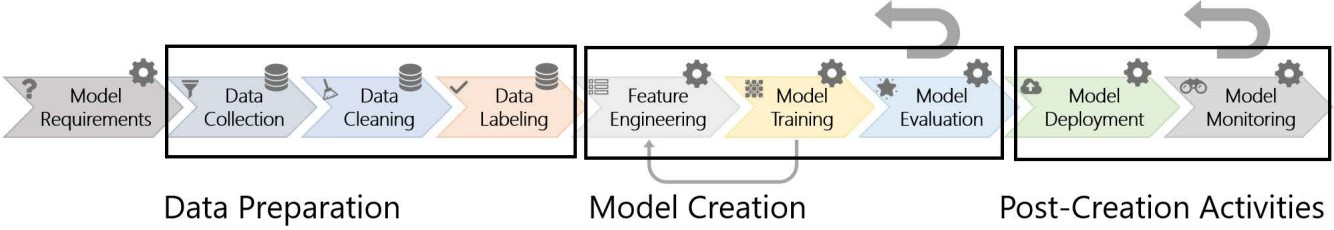
\includegraphics[width = \linewidth]{Monitoring/MLworkflow.jpg}
        \caption{ML workflow.}
    \end{figure}
\end{frame}
\subsection{\textit{2020 Draft \& Research Agenda} Towards a low-code solution for monitoring machine learning model performance}
\begin{frame}{Draft: data draft \& concept draft}
    \begin{itemize}
        \item 有监督学习中的X,Y通常被视为服从联合概率分布P(X, Y)的随机变量。由于真实世界情况复杂且不稳定,概率分布会发生变化,即概念漂移、采样漂移、先验概率漂移或更一般的数据集漂移。此处主要讨论数据漂移和概念漂移两种。
        \item data draft
        \begin{itemize}
            \item 数据漂移可能是由采样机制,环境中的未知因素随时间变化引起。
            \item 数据漂移不一定导致输出错误,没有数据漂移也不一定能保证输出正确。
            \item 目前可以通过检查数据输入来检测数据漂移。
        \end{itemize}
        \item concept draft
        \begin{itemize}
            \item 概念漂移指输入-输出映射发生变化。概念漂移可能是真实的,也可能是虚拟的。
            \item 真实:由于某些未知因素发生改变,导致映射发生改变;
            \item 虚拟:映射实际并没有发生改变,只是由于其它原因观测到这个现象(比如有偏采样)。
        \end{itemize}
    \end{itemize}
\end{frame}
\begin{frame}{Research Agenda}
    \begin{itemize}
        \item Data Capture
        \begin{itemize}
            \item 为了检测概念漂移,需要存储模型输出并与反馈进行对比
        \end{itemize}
        \item Algorithm Execution
        \begin{itemize}
            \item 希望能使用DSL来描述漂移检测算法,然后生成适用于不同框架的算法
        \end{itemize}
        \item Responding to Detected Drift
        \begin{itemize}
            \item 方法是多样的,可以包含以下两种
            \begin{itemize}
                \item data drift: 检测到漂移时简单地发送email
                \item concept drift: 自动触发重新训练模型的流程
            \end{itemize}
        \end{itemize}
    \end{itemize}
\end{frame}
% \begin{frame}{Survey}
%     \begin{itemize}
%         \item Review: work flow of ML
%         \item Problem
%         \begin{itemize}
%             \item key concepts: data drift, concept drift
%         \end{itemize}
%         \item Approach: furture research agenda
%         \begin{itemize}
%             \item Data capture
%             \item Algorithm execution
%             \item Responding to detected drift
%         \end{itemize}
%     \end{itemize}
% \end{frame}
\subsection{\textit{2021 Solution} A Model-Driven Engineering Approach for Monitoring Machine Learning Models}
\begin{frame}{Solution: Meta-Model}
    \begin{itemize}
        \item assumptions for model deployment
        \item 
    \end{itemize}
\end{frame}
\end{document}